%% Elsevier / Applied Soft Computing manuscript
%% Prepared with elsarticle numbered-reference template.
\documentclass[1p,times]{elsarticle}

\usepackage{cmap}
\usepackage[T1]{fontenc}
\usepackage[utf8]{inputenc}
\usepackage{lmodern}
\usepackage{amssymb}
\usepackage{amsmath}
\usepackage{booktabs}
\usepackage{array}
\usepackage{graphicx}
\usepackage{url}
\usepackage{enumitem}
\usepackage[protrusion=true,expansion=false]{microtype}
\usepackage{float}
\usepackage{longtable}
\usepackage{caption}
\usepackage{multirow}
\usepackage{tabularx}
\setlength{\emergencystretch}{3em}
\setlength{\textfloatsep}{8pt}
\setlength{\floatsep}{6pt}
\setlength{\intextsep}{6pt}
\captionsetup{font=small,skip=2pt}
\setlist{nosep,leftmargin=*}

\journal{Applied Soft Computing}
\biboptions{numbers}

\begin{document}

\begin{frontmatter}

\title{Selection-Filtered Predictive Redeployment for Rapid Recovery in Dynamic Multi-Objective Evolutionary Optimization}

\author[aff1]{Ercan Erkalkan\corref{cor1}}
\ead{ercan.erkalkan@marmara.edu.tr}

\cortext[cor1]{Corresponding author.}

\affiliation[aff1]{organization={Marmara University, Vocational School of Technical Sciences, Department of Computer Technologies},
            addressline={Mehmet Genc Kulliyesi},
            city={Kartal, Istanbul},
            postcode={34865},
            country={Turkey}}

\begin{abstract}
Soft-computing methods for dynamic multi-objective decision problems must adapt quickly while remaining robust to uncertainty in historical information and prediction reliability. Prediction can accelerate dynamic multi-objective evolutionary optimization, but it can also be harmful when environmental changes are abrupt, historical states are no longer informative, or the estimated movement direction is wrong. This paper proposes PRR-NSGA-II, a selection-filtered predictive redeployment strategy with bounded memory support that treats prediction as candidate generation rather than guaranteed population admission. After each change, predicted candidates are re-evaluated under the current objectives and must compete with elite, recent-memory, historical-transfer, and diversity candidates through NSGA-II environmental selection. The resulting design is a conservative candidate-admission mechanism: useful predictions can accelerate recovery, whereas inaccurate predictions are not allocated protected slots. Memory and elite preservation are likewise treated as candidate sources, not as guaranteed contributors, because stale historical information can become harmful in some regimes. The empirical study covers 20 dynamic scenarios, including FDA, dMOP, adapted DF-style, high-frequency/high-severity variants, and two application-inspired synthetic diagnostic cases for resource allocation and scheduling; these APP cases are not real-world validated datasets. The evaluation uses 30 independent runs, 10 algorithms, scenario-level rank aggregation, independent non-parametric tests with Holm correction and effect sizes, objective-evaluation accounting, direct recovery diagnostics, component-risk ablation, source-quota sensitivity, and a synthetic prediction-noise stress test. The results support a bounded claim. PRR-NSGA-II is competitive overall and is strongest on selected high-change regimes, especially high-frequency and application-inspired subsets, where conservative candidate admission remains effective for rapid redeployment. The ABR-inspired NSGA-II implementation remains the strongest overall adaptive response-family baseline in the controlled code base, particularly under high-severity and prediction-hostile conditions. Direct-insertion and no-memory/no-elite ablations expose boundary cases in which the complete fixed-quota PRR configuration is not the aggregate winner. PRR is therefore positioned not as a universal state-of-the-art replacement, but as a simpler, interpretable, and selection-safe soft-computing alternative for rapid recovery when prediction reliability varies across environments.
\end{abstract}



\begin{keyword}
soft computing \sep evolutionary computing \sep dynamic multi-objective optimization \sep predictive redeployment \sep memory archive \sep NSGA-II \sep decision stability
\end{keyword}

\end{frontmatter}

\section{Introduction}
Dynamic multi-objective optimization problems occur when objectives, constraints, decision variables, or environmental parameters change over time \cite{branke2002}. Farina et al. formalized representative dynamic multiobjective test cases and approximation issues \cite{farina2004}. Nguyen et al. later reviewed evolutionary dynamic optimization as a distinct research area \cite{nguyen2012}. The algorithm must therefore track a sequence of Pareto-optimal regions rather than solve one static problem. This requirement appears in adaptive scheduling, power systems, routing, control, and real-time decision support, where soft-computing methods are attractive because they can trade exactness for robustness, tractability, and low response cost under uncertainty. Recent adaptive-boosting work shows that the same issue remains active in current DMOO research \cite{peng2024ab}. A recent resource-allocation study also illustrates the practical relevance of dynamic multiobjective response \cite{hu2025resource}. In this paper, however, the two APP scenarios are application-inspired synthetic diagnostic cases rather than real-world validated datasets: they are included to expose resource-allocation and scheduling-like change patterns under controlled conditions, not to claim field validation. A population that is adequate before a change may become poorly located immediately after it; rapid recovery requires convergence, diversity, and useful historical information to be balanced under a limited evaluation budget.

Evolutionary multi-objective algorithms are natural candidates because they maintain multiple trade-off solutions, but static algorithms such as NSGA-II do not specify how the population should be redeployed after a change \cite{deb2002}. Dynamic responses have therefore evolved along several mechanism families: diversity injection, memory reuse, prediction of Pareto-set movement, transfer from related environments, and adaptive allocation among these sources \cite{yang2008,zhou2014,arms2022,peng2024ab,mstl2022}. Recent work increasingly combines these families through reference-vector prediction, pivot-point prediction, prediction archives, ensemble prediction, feature-fusion reinforcement learning, and interval-based historical response \cite{zheng2023rvcp,pivot2023hppds,wang2024dmpa,ensemble2024,li2025mffrl,ou2026hcips}. This creates a stricter standard for a new method: the contribution must be explained mechanistically against hybrid and adaptive response families, not only compared numerically with static or simple immigrant baselines.

From a soft-computing perspective, this paper addresses a narrower but methodologically important part of that question: how to combine imprecise prediction, historical memory, and diversity without giving any uncertain source privileged admission after a change. The contribution is not the mere coexistence of memory, prediction, and diversity, because current DMOEAs already combine such mechanisms. It is also not the claim that NSGA-II environmental selection itself is new. The proposed distinction is where prediction is admitted into the response pipeline. In PRR-NSGA-II, prediction generates hypotheses about the next useful region, but these hypotheses receive no guaranteed positions in the redeployed population. After a change, predicted solutions are re-evaluated in the new environment and must compete with elite survivors, bounded-memory samples, historical-transfer samples, and diversity immigrants under the same current-state selection rule. This design differs from deterministic prediction insertion, where a fixed number of predicted candidates is retained because it was predicted. The purpose is therefore conservative: retain the recovery benefit of temporal movement estimation when it is useful, but prevent inaccurate predictions from bypassing environmental selection. PRR-NSGA-II is consequently positioned as an interpretable, modular, and selection-safe redeployment strategy for rapid-recovery settings, not as a universal guarantee of state-of-the-art performance on every dynamic benchmark.

The main contributions are as follows:
\begin{enumerate}[leftmargin=*]
\item A selection-filtered redeployment rule is formulated as a conservative soft-computing candidate admission mechanism for rapid-recovery dynamic multi-objective evolutionary optimization.
\item A selection-safety design property is stated for harmful prediction: a predicted candidate has no reserved access to the next population when enough current-state alternatives have higher environmental selection priority. This property is explicitly framed as a consequence of the admission rule, not as an independent theorem about NSGA-II.
\item The method uses four candidate-generation blocks--elite, memory, prediction, and diversity--where the memory block is internally split into recent-memory and historical-transfer samples before current-state selection.
\item The difference between filtered candidate admission and deterministic prediction insertion is isolated through component-risk ablation with no-prediction, no-memory, no-diversity, no-elite, and direct-insertion variants.
\item The fixed PRR source ratios are treated as tunable design parameters rather than hidden constants; a targeted source-quota sensitivity audit and a prediction-noise stress test are reported.
\item Ten algorithms are compared on FDA, dMOP, adapted DF-style benchmark families, and two clearly labelled application-inspired synthetic diagnostics under an equal-generation rapid-response protocol, accompanied by an explicit function-evaluation audit, scenario-level rank aggregation, family-level diagnostics, scenario-normalized scores, and direct recovery measurements.
\end{enumerate}

The rest of the paper is organized as follows. Section 2 reviews related work. Section 3 formulates the problem and metrics. Section 4 presents PRR-NSGA-II. Section 5 describes the experimental protocol. Section 6 reports results, statistical analyses, ablation, and sensitivity analyses. Section 7 discusses limitations and threats to validity. Section 8 concludes the paper.

\section{Related Work}
\subsection{Dynamic multi-objective optimization}
Dynamic multi-objective optimization extends static multi-objective optimization by allowing objective landscapes, Pareto-optimal sets, constraints, or decision variables to vary over time. The area rests on classical Pareto trade-off concepts and evolutionary multiobjective foundations \cite{miettinen1999,deb2001,coello2007}, while early dynamic studies established the need for response mechanisms and state-wise evaluation \cite{branke2002,farina2004,nguyen2012}. For the present paper, the important lesson from benchmark and survey work is not simply that many test problems exist. It is that conclusions are sensitive to front geometry, decision-space movement, change frequency, severity, multimodality, and whether previous environments remain informative \cite{huband2006,li2009,helbig2014,benchmark2022xiang}. Recent constrained dynamic studies add another layer: when feasibility changes, the useful response may be different from the response that works in unconstrained tracking \cite{constrained2023dvc,asoc2024acrm,constrained2026dualpred,fgsp2025}. PRR is therefore evaluated as a rapid redeployment mechanism under controlled two-objective dynamics, not as a complete solution for every constrained or many-objective dynamic setting.

\subsection{Memory and diversity mechanisms}
Memory and diversity responses address opposite risks after a change. Memory can accelerate convergence when environments recur, but it can cause negative transfer when the archived solutions reflect obsolete regions. Diversity injection, including random immigrants and hypermutation, reduces that risk but may spend evaluations on uninformative exploration \cite{yang2008,nguyen2012}. These mechanisms are usually embedded in dominance- or decomposition-based hosts such as NSGA-II or MOEA/D \cite{deb2002,zhang2007,trivedi2017}. The recent transfer-learning literature makes the weakness of naive memory explicit: historical material must be selected, adapted, or rejected when the source and current environments differ \cite{mstl2022,domain2022,wu2023kt,li2024nitl,song2024mst,osbitp2025}. PRR follows this cautionary view. Recent-memory and historical-transfer candidates are not trusted by origin; they are re-evaluated in the current state and filtered together with prediction and diversity candidates.

\subsection{Prediction-assisted dynamic optimization}
Prediction-assisted dynamic optimization estimates movement in the Pareto set, objective space, reference directions, representative points, manifolds, or learned latent representations. Such prediction can substantially shorten recovery when the environmental trajectory is regular \cite{zhou2014,grey2020,objective2021,hybrid2022mutation}. Later variants enrich the prediction target or model class through classification, swarm adjustment, manifold learning, reference-vector prediction, pivot points, archives, ensembles, collaborative layers, feature transfer, and interval prediction \cite{classification2022,particle2022pspas,manifold2023mcp,zheng2023rvcp,pivot2023hppds,wang2024dmpa,ensemble2024,hu2025dlcp,ruan2026feature,ou2026hcips}. The common vulnerability is that prediction quality is state dependent. A predicted solution that is useful under smooth movement can be harmful under abrupt changes, high severity, or poorly converged historical states. PRR therefore does not reserve slots for predicted candidates. Prediction proposes search hypotheses, and environmental selection decides whether they are admitted.

Specialized DMOO settings reinforce the same design tension. Expensive dynamic optimization uses surrogates and transfer to reduce evaluations \cite{expensive2022kriging,expensive2025knee}; robust and constrained variants must account for uncertainty and moving feasibility regions \cite{robust2025pstl,constrained2023dvc,asoc2024acrm,constrained2026dualpred,fgsp2025}. These lines are not direct competitors to PRR, but they show why a response mechanism should state what kind of uncertainty it handles. PRR handles one specific uncertainty: whether a predicted or transferred candidate should be admitted after a change.

\subsection{Adaptive and hybrid response selection}
Adaptive and hybrid response methods address the allocation problem directly: how much effort should be assigned to memory, prediction, diversity, transfer, or other response operators after each change \cite{arms2022,peng2024ab,rsas2024}. Transfer-oriented methods address a related source-selection problem by deciding which historical material is likely to be useful \cite{mstl2022,domain2022,wu2023kt,li2024nitl,song2024mst,osbitp2025}. PRR is complementary rather than identical to these approaches. It uses fixed source quotas in the present study, so it is less adaptive than ABR-style allocation methods, but it adds a post-generation admission gate: no candidate source, including prediction, bypasses current-state selection. Table \ref{tab:mechanistic-comparison} summarizes this distinction in terms of memory use, prediction use, filtering, and negative-prediction handling.


\begin{table}[htbp]
\centering
\caption{Critical comparison of dynamic response families relative to PRR-NSGA-II. Mem. = uses memory; Pred. = uses prediction; Filter = has explicit selection filtering before admission; Neg. = handles harmful prediction or negative transfer. Y = yes, N = no, P = partial.}
\label{tab:mechanistic-comparison}
\scriptsize
\setlength{\tabcolsep}{2pt}
\renewcommand{\arraystretch}{1.18}
\begin{tabularx}{\linewidth}{p{0.20\linewidth}ccccX}
\toprule
Method family & Mem. & Pred. & Filter & Neg. & Difference from PRR \\
\midrule
Diversity/immigrant response & N & N & P & N & Improves exploration after a change, but does not exploit temporal movement or stored knowledge. \\
Memory/archive reuse & Y & N/P & P & P & Reuses prior solutions; PRR also re-evaluates memory and lets it compete against prediction, transfer, elite, and immigrants. \\
Transfer/knowledge reuse & Y & P & P & P & Selects or adapts historical material; PRR adds a common current-state admission gate for both transfer and prediction candidates. \\
Deterministic prediction insertion & P & Y & N & Weak & Predicted candidates occupy reserved response slots; PRR allows zero predicted candidates to survive when current-state selection rejects them. \\
Reference-vector or pivot prediction & P & Y & P & P & Guides search directions or representative points; PRR focuses on whether generated candidates are admitted into the redeployed population. \\
Adaptive boosting/response selection & Y & Y & P & P & Adapts source allocation and is often stronger overall; PRR is simpler and emphasizes post-generation filtering rather than adaptive quota learning. \\
Robust dynamic response & P & P & Y & P & Favors solutions stable under uncertainty; PRR targets rapid current-state recovery and reports decision drift separately. \\
PRR-NSGA-II & Y & Y & Y & Y & Prediction, memory, transfer, elite, and diversity candidates are re-evaluated under the current state and admitted only through environmental selection. \\
\bottomrule
\end{tabularx}
\end{table}

\subsection{Decision-oriented evaluation}
Dynamic optimization can also be viewed from a decision-support perspective \cite{hwang1981}. Outranking methods show why repeated compromise choice matters beyond pure approximation quality \cite{roy1996}. Modern MCDA surveys reinforce the same decision-oriented view \cite{greco2016}. A Pareto approximation is useful not only when it is close to the front, but also when compromise alternatives remain stable enough to support repeated decisions. For this reason, this study reports hypervolume and IGD together with stability, decision drift, and a quality-drift ratio. Hypervolume is a widely used convergence-diversity indicator \cite{zitzler1999}. Efficient hypervolume computation further supports its practical use in empirical comparison \cite{fonseca2006}. Statistical comparisons follow non-parametric testing recommendations for evolutionary computation \cite{derrac2011}. Effect-size interpretation is added so that significance is not treated as the only evidence of practical difference \cite{sawilowsky2009}.




\section{Problem Formulation and Evaluation Metrics}
Let $X \subseteq [0,1]^n$ be the decision space and let $t=0,\ldots,T-1$ denote a discrete environmental state. This zero-based state convention matches the supplementary benchmark definitions and the implementation loop; the first environment is $t=0$ and the last is $t=T-1$. A dynamic multi-objective minimization problem is defined as
\begin{equation}
\min F(x,t)=\left(f_1(x,t),f_2(x,t),\ldots,f_m(x,t)\right), \quad x \in X.
\end{equation}
A solution $x_a$ dominates $x_b$ at time $t$ if $f_i(x_a,t)\leq f_i(x_b,t)$ for all objectives and the inequality is strict for at least one objective. The algorithm seeks to approximate the Pareto front $PF(t)$ for each state while reducing the recovery delay after changes.

The study uses five metrics. Hypervolume (HV) measures the dominated objective-space volume with respect to a reference point; higher values are better \cite{zitzler1999}. Efficient computation procedures support the use of HV in empirical comparison \cite{fonseca2006}. Because the FDA, dMOP, adapted DF-style, and application-inspired cases have different objective ranges, HV is normalized by a scenario-level reference rectangle generated from the state-wise reference sets. Inverted generational distance (IGD) measures the average distance from reference-set points to the obtained non-dominated approximation; lower values are better \cite{coello2007}. For FDA, dMOP, and adapted DF-style cases, the reference sets are generated from the analytic or constructed dynamic front definitions listed in Supplementary Section S1. For APP-RESOURCE and APP-SCHEDULING, the sets are best-known diagnostic reference traces generated from the time-varying target structure rather than analytically proven true Pareto fronts; APP IGD is therefore interpreted as a diagnostic indicator and not as proof of convergence to a closed-form true front. Each state-wise reference set contains 300 points. Stability is defined as
\begin{equation}
S = \frac{1}{1+\frac{1}{T-1}\sum_{t=1}^{T-1}|HV_t-HV_{t-1}|},
\end{equation}
where a higher value indicates smoother quality variation. Decision drift is computed as the mean Euclidean distance between consecutive compromise solutions selected by normalized distance to the ideal point; lower values indicate more stable compromise decisions. This ideal-point compromise logic is consistent with classical multi-attribute decision-making concepts \cite{hwang1981}.
Because drift alone can reward poor but immobile approximations, the study also reports a quality-drift ratio:
\begin{equation}
QDR = \frac{\overline{HV}}{1+\overline{D}},
\end{equation}
where $\overline{HV}$ is the mean normalized hypervolume over environmental states and $\overline{D}$ is the mean decision drift. Higher QDR values indicate a better balance between approximation quality and compromise-solution movement.

\section{Proposed PRR-NSGA-II Method}
\subsection{General architecture}
Figure \ref{fig:architecture} summarizes the method. After a change, PRR-NSGA-II forms a redeployment pool from four candidate-generation blocks: elite survivors, a memory block, prediction-guided candidates, and random immigrants. The memory block is internally split into recent-memory and historical-transfer samples, but both sub-blocks are tracked under the memory quota in the implementation and diagnostics. The pool is evaluated under the current environment and selected through NSGA-II-style environmental selection.

\begin{figure}[htbp]
\centering
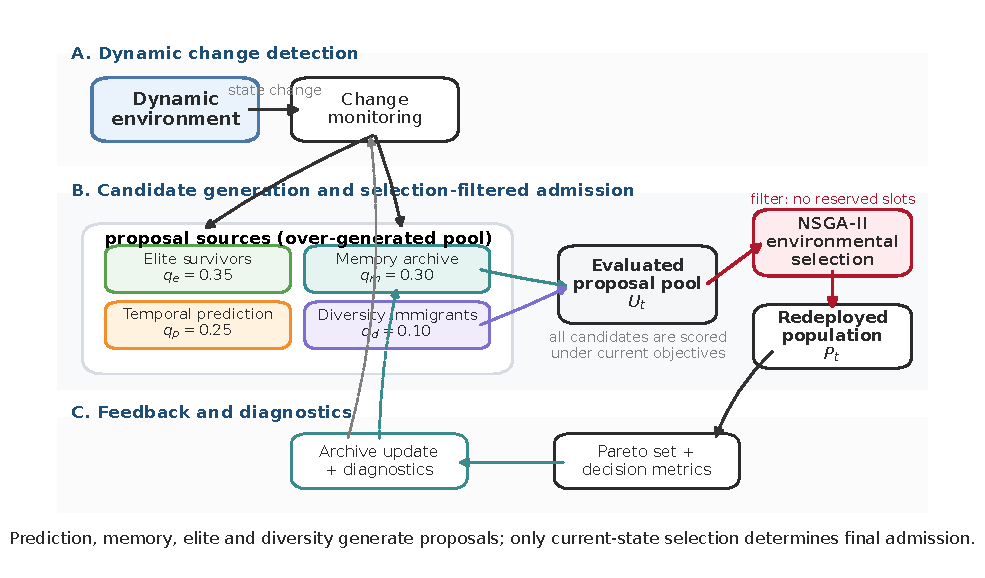
\includegraphics[width=\linewidth]{figure1_architecture.pdf}
\caption{Architecture of PRR-NSGA-II. Predicted candidates compete with elite, diversity, and memory-block candidates; the memory block is internally split into recent-memory and historical-transfer samples. Final redeployment is controlled by current-state selection.}
\label{fig:architecture}
\end{figure}

\subsection{Memory archive}
At each state, a bounded archive stores non-dominated or high-quality solutions. The memory is updated by selecting at most $K$ solutions from the union of the previous memory and the current non-dominated set using non-dominance and diversity ranking. During redeployment, the memory component is split between recent archive samples and historical-transfer samples. The latter are sampled from previous non-dominated archives with a recency bias and perturbed mildly. This allows PRR-NSGA-II to reuse earlier environments without copying all historical individuals into the new population.

\subsection{Temporal movement estimation}
Let $M_t$ be the memory archive at environmental state $t$. The decision-space centroid is
\begin{equation}
c_t = \frac{1}{|M_t|}\sum_{x\in M_t}x.
\end{equation}
The implementation parameter $w$ denotes the number of most recent valid archive centroids retained for prediction, not the number of displacement vectors. Let
\[
\mathcal{C}^{(w)}_t=(c_{\tau_1},\ldots,c_{\tau_m}), \qquad m\leq w,
\]
be these centroids in chronological order after empty archives are skipped. The temporal movement vector is computed from the $m-1$ available consecutive centroid differences:
\begin{equation}
\hat{v}_{t+1}=\sum_{j=1}^{m-1}\beta_j(c_{\tau_{j+1}}-c_{\tau_j}), \quad \sum_{j=1}^{m-1}\beta_j=1, \quad \beta_j\geq 0.
\end{equation}
If fewer than two valid centroids are available, the implementation falls back to random immigrants or mutation around the latest valid archive rather than computing a displacement vector. Thus, the default $w=4$ uses at most four recent centroids and therefore at most three displacement vectors. Prediction-guided candidates are generated by
\begin{equation}
x_i^{pred}=\mathrm{clip}\left(x_i+\lambda\hat{v}_{t+1}+\epsilon_i,0,1\right),
\end{equation}
where $x_i$ is sampled from memory, $\lambda$ is a scale factor, and $\epsilon_i$ is a small mutation term.

\subsection{Selection-filtered redeployment as conservative candidate admission}
Let $\mathcal{S}^{t}_{N}(A)$ denote NSGA-II environmental selection of $N$ candidates from a finite set $A$ after evaluating every candidate under the current environment $t$. Selection is ordered first by non-dominated rank under $F(\cdot,t)$ and then by crowding distance. The important design choice in PRR-NSGA-II is not to modify this environmental-selection rule, but to postpone admission until all response sources have produced candidates and all candidates have been re-evaluated in the current environment. For a population size $N$, the redeployment union is
\begin{equation}
U_t=P^{elite}_t\cup P^{recent}_t\cup P^{trans}_t\cup P^{pred}_t\cup P^{div}_t.
\end{equation}
Here $P^{recent}_t\cup P^{trans}_t$ is the internally split memory block: $P^{recent}_t$ is sampled from the latest archive and $P^{trans}_t$ from previous non-dominated archives. Both sub-blocks are assigned the same memory source label in the implementation. The PRR redeployment rule is
\begin{equation}
P^{PRR}_t=\mathcal{S}^{t}_{N}(U_t).
\end{equation}
The accepted number of predicted candidates is therefore an outcome of current-state selection rather than a user-set quota:
\begin{equation}
a^{pred}_t=\left|P^{PRR}_t\cap P^{pred}_t\right|,\quad 0\leq a^{pred}_t\leq |P^{pred}_t|.
\end{equation}
This definition is the core difference from direct prediction insertion. A direct-insertion response with a fixed prediction quota $q$ can be written as
\begin{equation}
P^{DIR}_t=Q^{pred}_t\cup \mathcal{S}^{t}_{N-q}\left(U_t\setminus Q^{pred}_t\right),\quad Q^{pred}_t\subseteq P^{pred}_t,\quad |Q^{pred}_t|=q.
\end{equation}
In $P^{DIR}_t$, the members of $Q^{pred}_t$ enter the redeployed population because they are predicted. In $P^{PRR}_t$, a predicted candidate enters only if it remains competitive after current-state evaluation. Thus, prediction is used as a proposal mechanism rather than as an admission privilege.

\textit{Conservative admission property.} Let $x\in P^{pred}_t$ be a predicted candidate whose current-state priority after re-evaluation is poor. If at least $N$ candidates in $U_t\setminus\{x\}$ have better environmental selection priority than $x$, then $x\notin P^{PRR}_t$. This statement follows directly from the definition of $\mathcal{S}^{t}_{N}$, which selects the $N$ highest-priority candidates from the evaluated union. It is therefore not presented as a new theorem about NSGA-II. Its role is to make explicit the admission safeguard created by PRR: inaccurate predicted candidates cannot bypass current-state selection merely because they came from the prediction operator. Direct insertion does not satisfy the same admission condition because any $x\in Q^{pred}_t$ is retained by construction, even when its current-state dominance rank and crowding priority are poor.

This property does not imply that PRR must obtain a larger HV or smaller IGD than direct insertion in every smooth or highly predictable environment. If prediction is accurate, reserved insertion can be effective. The expected advantage of filtered admission is instead in mixed, abrupt, or high-frequency settings where prediction can be useful for recovery but risky enough that hard admission quotas may introduce negative transfer into the new population.

\paragraph{Toy clarification of the distinction.}
Consider a response step with population size $N=4$. Suppose the evaluated response pool contains four strong current-state candidates, $e_1$, $m_1$, $d_1$, and $e_2$, generated by elite, memory, diversity, and elite sources, and two predicted candidates, $p_1$ and $p_2$, that are poor after the environmental change. Under current-state environmental selection, the priority order is
\[
 e_1 \succ m_1 \succ d_1 \succ e_2 \succ p_1 \succ p_2,
\]
where $a\succ b$ means that $a$ has higher NSGA-II environmental-selection priority after re-evaluation in the new environment. A direct-insertion response with a reserved prediction quota $q=2$ can admit $p_1$ and $p_2$ before the remaining two slots are filled from other sources. PRR-NSGA-II instead applies $\mathcal{S}^{t}_{4}$ to the entire evaluated union, yielding $\{e_1,m_1,d_1,e_2\}$ and rejecting both predicted candidates. If a predicted candidate were truly useful, for example if $p_1\succ d_1$, it would be admitted by the same rule. Thus, PRR does not reject prediction; it rejects \emph{admission privilege}. Prediction is treated as a candidate proposal source whose output must survive the same current-state selection test as every other source.

The practical implementation therefore distinguishes \emph{generation quotas} from \emph{admission quotas}. Let the nominal source-share vector be
\begin{equation}
(q_e,q_m,q_p,q_d)=(0.35,0.30,0.25,0.10),
\end{equation}
for elite, memory, prediction, and diversity, respectively. These values determine how many candidates are proposed by each source before filtering, not how many candidates are guaranteed to enter the next population. To make filtering non-vacuous, PRR builds an over-generated response pool of size
\begin{equation}
|U_t|=\rho_{\mathrm{pool}} N,\quad \rho_{\mathrm{pool}}=2.0,
\end{equation}
and then selects only $N$ candidates from $U_t$ after current-state evaluation. Thus, approximately $0.70N$ elite-derived, $0.60N$ memory-derived, $0.50N$ prediction-derived, and $0.20N$ diversity-derived candidates compete for $N$ positions under the default configuration. The accepted source fractions are consequently measured outcomes, not fixed quotas. The values above are intentionally conservative defaults: elite and memory preserve continuity, prediction supplies directed recovery, and diversity keeps a small exploratory reserve. Section 6 reports a targeted source-quota sensitivity audit rather than treating these ratios as universally optimal.

The implementation records these measured admission outcomes explicitly. The PRR response routine attaches a source label to every generated candidate and, after environmental selection, logs the proposed count, accepted count, acceptance fraction, and final-population fraction for elite, memory, prediction, and diversity sources. The manuscript package includes the generated files \path{04_supplementary_material/results/prr_source_diagnostics_raw.csv}, \path{04_supplementary_material/results/prr_source_diagnostics_by_scenario.csv}, and \path{04_supplementary_material/results/prr_source_diagnostics_overall.csv}; they can be regenerated with \path{04_supplementary_material/src/run_prr_source_diagnostics.py} or the \texttt{source-diagnostics} command-line mode.

Memory is also split explicitly. At the end of state $t$, the archive is updated from the current state's non-dominated population, then truncated to $K=100$ by current-state environmental selection. The archive therefore stores decision vectors but is filtered using the objective values of the environment in which the update is performed. At the next change response, the memory block is divided into recent-memory and historical-transfer sub-blocks:
\begin{equation}
|P^{recent}_t|=\lceil \eta |P^{mem}_t|\rceil,\quad |P^{trans}_t|=|P^{mem}_t|-|P^{recent}_t|,\quad \eta=0.55.
\end{equation}
Recent-memory candidates are sampled from the bounded archive of the immediately preceding state. Historical-transfer candidates are sampled from the sequence of previous non-dominated archives with linear recency weights
\begin{equation}
\omega_j=\frac{0.35+(j-1)(1.0-0.35)/(h-1)}{\sum_{\ell=1}^{h}\left[0.35+(\ell-1)(1.0-0.35)/(h-1)\right]},
\end{equation}
where $j=1$ denotes the oldest available archive and $j=h$ the most recent. Transfer candidates are perturbed by Gaussian noise with standard deviation $0.5\sigma$, predicted candidates by $0.7\sigma$, and offspring mutation uses $\sigma=0.07$ with per-variable probability $1/D$. All memory, transfer, and prediction candidates are re-evaluated under the current state before admission.

The selection-filter also provides a simple contamination bound relative to direct insertion. Suppose a direct-insertion response reserves $q$ predicted positions and $H_t\subseteq P^{pred}_t$ denotes harmful predicted candidates whose current-state priority is worse than the $N$th best non-predicted candidate available in $U_t$. Direct insertion can retain as many as $\min(q,|H_t|)$ harmful predictions because the quota is reserved before environmental selection. PRR has no such lower bound: the number of harmful predictions admitted is
\begin{equation}
c^{PRR}_t=\left|H_t\cap \mathcal{S}^{t}_{N}(U_t)\right|,
\end{equation}
which is zero whenever $N$ non-predicted or non-harmful candidates have higher current-state priority. The bound is intentionally modest but useful: PRR cannot make a wrong prediction harmless, but it can prevent wrong predictions from receiving protected admission. This is why the stress test in Section 6 varies prediction noise and compares accepted predicted candidates against a direct-insertion quota.

\subsection{Pseudo-code}
Table \ref{tab:pseudocode} gives the implementation-level sequence used by the reference code, including the accepted-source diagnostic output.
\begin{table}[htbp]
\centering
\caption{PRR-NSGA-II pseudo-code.}
\label{tab:pseudocode}
\begin{tabular}{p{0.94\linewidth}}
\toprule
\textbf{Input:} population size $N$, memory size $K$, states $T$, generations per state $G$, prediction history length $w$ (recent centroids), source shares $(q_e,q_m,q_p,q_d)$, pool multiplier $\rho_{\mathrm{pool}}$, recent-memory split $\eta$. \\
1. Initialize a working population $P^{init}\sim U(0,1)^D$ and an empty bounded archive history. \\
2. For each environmental state $t=0,\ldots,T-1$: \\
\quad 2.1. If $t=0$, use $P^{init}$ as the starting population; if $t>0$, compute source counts $n_s=\mathrm{round}(\rho_{\mathrm{pool}} Nq_s/\sum_s q_s)$ for $s\in\{e,m,p,d\}$. \\
\quad 2.2. For $t>0$, generate $P^{elite}_t$ by current-state selection from $P_{t-1}$; sample $P^{recent}_t$ from the latest archive; sample $P^{trans}_t$ from older archives with recency weights; generate $P^{pred}_t$ from centroid displacement; generate $P^{div}_t$ uniformly. \\
\quad 2.3. For $t>0$, perturb transfer and prediction candidates, clip them to $[0,1]^D$, and evaluate every candidate in $U_t=P^{elite}_t\cup P^{recent}_t\cup P^{trans}_t\cup P^{pred}_t\cup P^{div}_t$ under the current environment. \\
\quad 2.4. For $t>0$, set the redeployed population to $\mathcal{S}^{t}_{N}(U_t)$; no source, including prediction, receives a reserved admission slot. Record the proposed and accepted source-label counts for the selected $N$ candidates. \\
\quad 2.5. Run $G$ generations of blend crossover, Gaussian mutation, evaluation, and NSGA-II environmental selection in state $t$. \\
\quad 2.6. Set $P_t$ to the selected current population, update $M_t$ from its current-state non-dominated solutions, truncate the archive to $K$ solutions, and append it to the historical archive list. \\
3. Return the dynamic approximation sequence, metric values, and accepted-source diagnostic tables. \\
\bottomrule
\end{tabular}
\end{table}

\section{Experimental Protocol}
\subsection{Benchmark scenarios}
The main experiment uses transparent dynamic benchmark definitions rather than code-only descriptions. FDA1--FDA3 follow the classical FDA-style dynamic test-problem family \cite{farina2004}. dMOP1--dMOP3 follow the dMOP-style cases used in competitive-cooperative dynamic multi-objective studies \cite{goh2009}. DF1--DF5 are reported as adapted DF-style/CEC-DF-inspired two-objective cases: they preserve common dynamic-front motifs from the CEC'2018 benchmark family \cite{jiang2018cec}, but the implementation uses simplified formulas and is not claimed to be a bitwise reproduction of the official CEC'2018 definitions. The suite also includes high-frequency, low-frequency, and high-severity variants: FDA1-HF, FDA1-HS, dMOP2-LF, dMOP2-HS, DF1-HF, DF4-HS, and DF5-HF. Two application-inspired cases, APP-RESOURCE and APP-SCHEDULING, are included only as synthetic diagnostic cases. They model resource-allocation-like and scheduling-like trade-offs through normalized time-varying demand, price, urgency, lateness, and disruption terms, but they are not calibrated to operational data and should not be interpreted as real-world validated datasets. The complete objective formulas, dynamic parameters, variable bounds, and reference-set generation rules are provided in Supplementary Section S1 and in \path{src/dynamic_prr_experiment.py}; Tables \ref{tab:benchmark-suite} and \ref{tab:reference-status} summarize the family coverage and reference-set status.

The APP parameterization is intentionally simple and bounded. All decision variables remain in $[0,1]$ to match the rest of the benchmark suite. In APP-RESOURCE, a moving allocation target shifts around a mid-range operating point and a time-varying price multiplier changes the cost-emissions trade-off; this mimics a stylized setting in which demand and price drift over a planning horizon. In APP-SCHEDULING, urgency, target completion profiles, lateness, and disruption penalties vary with the environmental state; this mimics a stylized rescheduling setting in which the preferred activity profile and the cost of delay change over time. The coefficients are chosen to keep objective magnitudes comparable to the other diagnostic cases and to create interpretable smooth-plus-oscillatory movement, not to fit any particular industrial dataset.

\begin{table}[htbp]
\centering
\caption{Benchmark families used in the main experiment.}
\label{tab:benchmark-suite}
\small
\begin{tabular}{p{0.20\linewidth}p{0.38\linewidth}p{0.32\linewidth}}
\toprule
Family & Main cases & Stress variants \\
\midrule
FDA & FDA1, FDA2, FDA3 & FDA1-HF, FDA1-HS \\
dMOP & dMOP1, dMOP2, dMOP3 & dMOP2-LF, dMOP2-HS \\
Adapted DF-style & DF1, DF2, DF3, DF4, DF5 & DF1-HF, DF4-HS, DF5-HF \\
Application-inspired & APP-RESOURCE, APP-SCHEDULING & -- \\
\bottomrule
\end{tabular}
\end{table}


\begin{table}[htbp]
\centering
\caption{Reference-set and benchmark-definition status. This table prevents adapted or diagnostic cases from being interpreted as unqualified official test problems or as real-data validation cases.}
\label{tab:reference-status}
\small
\begin{tabular}{p{0.23\linewidth}p{0.31\linewidth}p{0.35\linewidth}}
\toprule
Family & Formula status & Reference-set status \\
\midrule
FDA & FDA-style formulas with state-dependent Pareto-set or front movement & Analytic or constructed state-wise front from the formula \\
dMOP & dMOP-style formulas with exponent, location, or decision-index movement & Analytic or constructed state-wise front from the formula \\
Adapted DF-style & CEC-DF-inspired simplified formulas; not official bitwise CEC'2018 cases & Constructed state-wise front implied by the implemented formula \\
Application-inspired & Purpose-built resource and scheduling trade-off models & Best-known diagnostic target traces; APP IGD is interpreted as diagnostic, not as a proof of true-front convergence \\
\bottomrule
\end{tabular}
\end{table}

\subsection{Algorithms and parameters}
Ten methods are compared: NSGA-II, DNSGA-II, MNSGA-II, PPS-NSGA-II, DMOEA/D, ARVLP-NSGA-II, KTR-NSGA-II, ABR-NSGA-II, RDMOEA-NSGA-II, and PRR-NSGA-II. The compact labels ARVLP-NSGA-II, KTR-NSGA-II, and ABR-NSGA-II are used in tables for readability, but throughout this manuscript they denote ARVLP-inspired, KTR-inspired, and ABR-inspired response-family implementations in the common NSGA-II-based experimental code base. They should not be read as exact source-code reproductions of the original authors' software. NSGA-II is the static baseline \cite{deb2002}. DNSGA-II and MNSGA-II represent immigrant and memory response families. PPS-NSGA-II tests the closest direct population-prediction alternative to selection-filtered prediction. DMOEA/D uses decomposition-based environmental selection \cite{zhang2007}. The decomposition-survey perspective informs this baseline family \cite{trivedi2017}. The ARVLP-inspired implementation tests linear population/reference-vector movement prediction \cite{zheng2023rvcp}. The KTR-inspired implementation tests selective historical knowledge-transfer response mechanisms \cite{wu2023kt}. Non-inductive transfer learning informs the selective-transfer interpretation of this baseline \cite{li2024nitl}. The ABR-inspired implementation tests adaptive allocation among memory, prediction, and diversity strategies \cite{peng2024ab}. Adaptive response allocation provides the broader response-selection basis for this baseline \cite{arms2022}. RDMOEA-NSGA-II represents robust dynamic response with a temporal-neighborhood mean-plus-dispersion objective. This design is motivated by robust dynamic optimization \cite{robust2025pstl}. Expensive-DMOO surrogate baselines are not included because all benchmark functions in this study are inexpensive and fully observable.

The comparison is now framed as a controlled response-family comparison rather than as a claim of bitwise reproduction. Table \ref{tab:config} lists the common experimental configuration.  All baselines are implemented in the same Python code base, use the same benchmark definitions, variation pipeline, population size, variable bounds, state sequence, and main equal-generation protocol, and apply their stated response mechanisms at every environmental change. Table \ref{tab:baseline-transparency} summarizes the implemented response families, source quotas, and post-response selection rules. The full pseudocode and fixed-parameter details for the three strongest recent response-family implementations are moved to the supplementary file \texttt{baseline\_implementation\_details.pdf}, while Table \ref{tab:baseline-transparency} keeps the main-text comparison auditable. This addition is intended to prevent the baselines from being read as opaque or selectively weakened variants. At the same time, the paper does not claim that ARVLP-NSGA-II, KTR-NSGA-II, ABR-NSGA-II, or the other baselines are exact source-code reproductions of their original papers. They are transparent single-codebase response-family implementations used to isolate mechanism-level differences under a common host algorithm, benchmark suite, and variation pipeline. Because response operators can require different numbers of current-state objective evaluations, the manuscript also distinguishes the equal-generation protocol from strict equal-function-evaluation budgeting.


\begin{table}[htbp]
\centering
\caption{Implementation transparency for compared methods. The baselines are reproducible response-family implementations in one code base, not bitwise source-code reproductions of all original papers.}
\label{tab:baseline-transparency}
\scriptsize
\setlength{\tabcolsep}{3pt}
\renewcommand{\arraystretch}{1.08}
\resizebox{\textwidth}{!}{%
\begin{tabular}{p{0.15\linewidth}p{0.23\linewidth}p{0.35\linewidth}p{0.18\linewidth}}
\toprule
Method & Response family tested & Change-response quota in this implementation & Selection after response \\
\midrule
NSGA-II & Static baseline & No explicit response & NSGA-II selection during evolution \\
DNSGA-II & Diversity immigrants & $0.75N$ selected survivors + $0.25N$ random immigrants & Survivor part filtered; immigrants inserted \\
MNSGA-II & Memory reuse & $0.65N$ selected survivors + up to $0.35N$ archive samples & Survivor part filtered; memory inserted \\
PPS-NSGA-II & Direct prediction insertion & $0.60N$ selected survivors + $0.40N$ predicted candidates & Predicted candidates have reserved admission \\
DMOEA/D & Decomposition response & $0.60N$ base + $0.15N$ memory + $0.15N$ prediction + $0.10N$ diversity & Weighted-sum scalar reselection \\
ARVLP-inspired NSGA-II & Linear/reference-vector prediction & $0.50N$ base + $0.40N$ linear prediction + $0.10N$ diversity & NSGA-II selection of response pool \\
KTR-inspired NSGA-II & Knowledge transfer & $0.45N$ base + $0.35N$ transfer + $0.20N$ prediction & NSGA-II selection of response pool \\
ABR-inspired NSGA-II & Adaptive response allocation & $0.35N$ elite + adaptive allocation of $0.65N$ among memory, prediction, and diversity pools & NSGA-II selection of scored response pool \\
RDMOEA-NSGA-II & Robust dynamic response & $0.65N$ robust base + $0.25N$ memory + $0.10N$ diversity & NSGA-II-style selection on robust objectives \\
PRR-NSGA-II & Selection-filtered redeployment & $2N$ generated pool: $0.70N$ elite + $0.60N$ memory/transfer + $0.50N$ prediction + $0.20N$ diversity; then select $N$ & NSGA-II selection of complete current-state pool; no source has reserved admission \\
\bottomrule
\end{tabular}%
}
\end{table}



All algorithms use the same population size, variable bounds, environmental states, and number of evolutionary generations per state. The common variation operator uses arithmetic blend crossover with probability $0.90$, Gaussian mutation with scale $\sigma=0.07$, mutation probability $1/D$, clipping to $[0,1]^D$, and one offspring population per generation. The archive cap is $100$ nondominated solutions for all memory-using methods. DMOEA/D and RDMOEA-NSGA-II use the same variation structure but intentionally reduce the search mutation scale to $0.85\sigma$ and $0.75\sigma$, respectively, to match their decomposition and robust-response roles. No per-scenario tuning is performed: quotas and hyperparameters are fixed before all runs. The ABR-inspired implementation is the exception only in the intended sense that its non-elite response quota is allocated online among memory, prediction, and diversity according to current-state candidate scores. The main experiment uses 30 independent runs, population size $100$, 10 decision variables, 20 environmental states, and 3 generations per state. This is an equal-generation rapid-response protocol, not a strict equal-function-evaluation protocol. The distinction matters because adaptive response mechanisms such as the ABR-inspired implementation and robust temporal-neighborhood selection can evaluate additional candidate pools during the change-response step. The supplementary evaluation-count audit therefore reports explicit objective-evaluation accounting. The main performance table is retained as the equal-generation comparison, while the rank, family, normalized-score, and recovery analyses are used as the primary interpretation layer. A separate sensitivity analysis evaluates 3, 5, 10, and 20 generations per state.

\begin{table}[htbp]
\centering
\caption{Main experimental configuration.}
\label{tab:config}
\begin{tabular}{lc}
\toprule
Parameter & Value \\
\midrule
Independent runs & 30 \\
Population size & 100 \\
Decision variables & 10 \\
Environmental states & 20 \\
Generations per state & 3 \\
Scenarios & 20 \\
Compared methods & 10 \\
Memory size & 100 \\
Prediction history length (recent centroids) & 4 \\
Prediction scale & 0.85 \\
PRR source shares $(q_e,q_m,q_p,q_d)$ & $(0.35,0.30,0.25,0.10)$ \\
PRR pool multiplier $\rho_{\mathrm{pool}}$ & 2.0 \\
Recent-memory split $\eta$ & 0.55 \\
\bottomrule
\end{tabular}
\end{table}

\subsection{Statistical testing}
The statistical protocol is deliberately conservative about pairing. The reference implementation uses deterministic algorithm-specific stochastic streams in the main stored results, so a run number is not treated as a natural paired block across algorithms. The Friedman test is therefore applied to scenario-level mean blocks rather than to artificially paired scenario-run blocks. Pairwise PRR-versus-baseline comparisons use two-sided Mann--Whitney tests with Holm correction instead of paired Wilcoxon tests. Cliff's delta is reported as an effect-size indicator \cite{sawilowsky2009}; for IGD and decision drift its sign is reversed so that positive values always favor PRR. The supplementary package contains per-scenario summaries, scenario-level average ranks, scenario-normalized scores, Holm-adjusted pairwise tests, win/tie/loss counts, and the evaluation-count audit.

\section{Results}
\subsection{Overall performance}
The result presentation is ordered to avoid over-interpreting a single grand mean. Table \ref{tab:average-ranks} gives the scenario-level average ranks and is treated as the main multi-scenario aggregation. The supplementary diagnostic CSV files then list the individual scenarios where PRR-NSGA-II ranks first, aggregate results by benchmark family, and separate high-frequency, high-severity, decision-space movement, application-inspired, prediction-filter-friendly, and prediction-hostile profiles. Table \ref{tab:overall} is still reported for transparency, but it is interpreted as an equal-generation overall mean rather than as the only evidence of performance.

Under the equal-generation protocol, the ABR-inspired implementation obtains the best overall mean for normalized HV, IGD, stability, and QDR. PRR-NSGA-II is the closest competitor on these four metrics and remains clearly ahead of the static, immigrant, memory-only, decomposition, transfer, and robust-response baselines. Scenario-level ranks give a more nuanced view: PRR has the best HV rank (2.30) and the best stability rank (3.80), while the ABR-inspired implementation has the best IGD and QDR ranks. The scenario-normalized score summary tells the same story without letting IGD scale differences dominate the average: the ABR-inspired implementation remains slightly ahead on HV/IGD/QDR scores, while PRR remains close and interpretable. Thus the main empirical claim is not that PRR is the universal winner, but that it provides a simpler, selection-safe admission-control alternative that stays near the ABR-inspired implementation overall and becomes preferable in identifiable rapid-recovery profiles.

Figure~\ref{fig:overall-metrics-panel} adds a compact visual summary of the five main indicators so that the manuscript is not read only through tables. Instead of separating HV and IGD into sparse standalone pages, the multi-panel layout shows the relative positions of PRR, the ABR-inspired implementation, and the remaining baselines across approximation quality, quality-drift balance, stability, and decision movement in one place. The figure makes the same interpretation visually explicit: ABR leads the overall means on HV, IGD, stability, and QDR, PRR remains the closest overall competitor, PRR ranks first on HV and stays competitive on stability, and both methods are clearly separated from the weaker baselines.

\begin{figure*}[t]
\centering
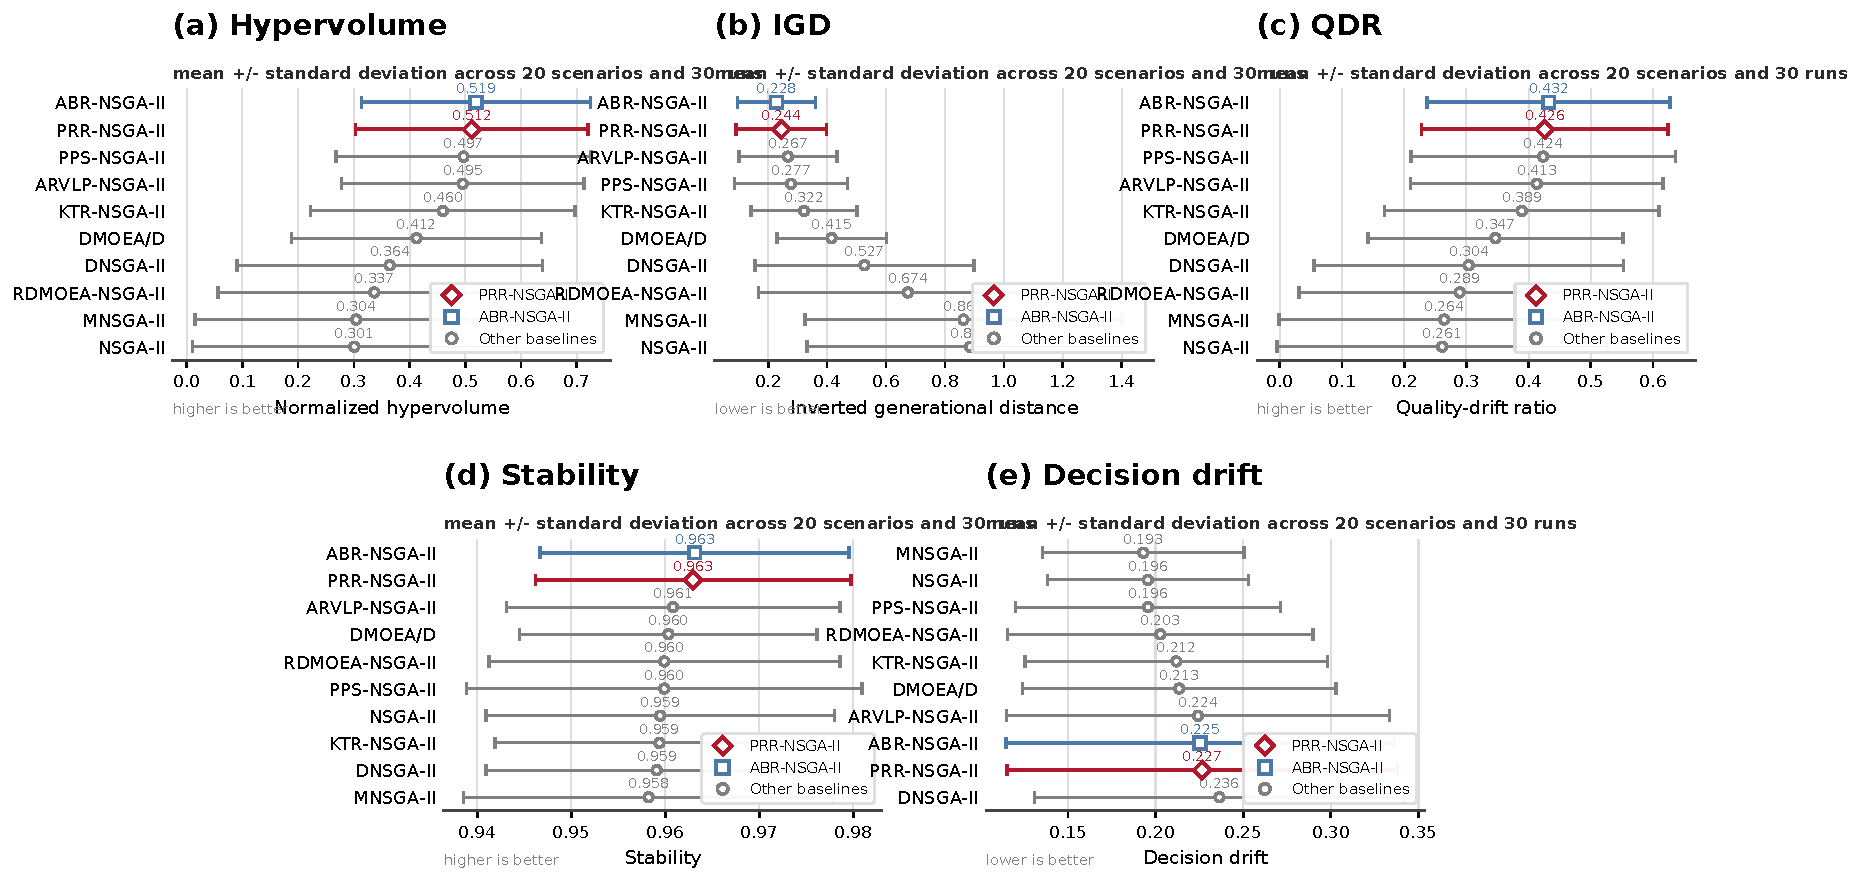
\includegraphics[width=\textwidth]{overall_metrics_panel.pdf}
\caption{Compact visual summary of the five main overall indicators under the equal-generation protocol. Panels report mean $\pm$ standard deviation across 20 scenarios and 30 runs for normalized HV, IGD, QDR, stability, and decision drift. Higher is better for HV, QDR, and stability; lower is better for IGD and decision drift. The multi-panel layout is used to show the overall empirical profile without spreading the main indicators across multiple sparse pages.}
\label{fig:overall-metrics-panel}
\end{figure*}

The evaluation-count audit is included to address budget fairness directly, rather than leaving this issue only in the supplementary material. It shows that response-heavy algorithms perform more objective-vector evaluations in the reference implementation than simple static or immigrant baselines. Therefore, the paper does not describe the main comparison as strict equal-function-evaluation superiority. Table~\ref{tab:fe-robustness} makes this accounting visible in the main text. The table should be read as an FE-accounting robustness check for the equal-generation protocol, not as a substitute for a complete FE-capped rerun. It is nevertheless useful for bounding the claim: PRR-NSGA-II is close to the ABR-inspired implementation while using fewer objective-vector evaluations, substantially outperforms the much more expensive RDMOEA-NSGA-II, but also uses more evaluations than PPS-NSGA-II, the ARVLP-inspired and KTR-inspired implementations, and the simpler NSGA-II variants. Thus, the appropriate conclusion is competitive and selection-safe rapid recovery under an equal-generation protocol, with strict FE-capped superiority left as a separate robustness experiment. The supplied code implements this audit through an \texttt{EvaluationCounter} hook inside \texttt{eval\_objectives()}. The dedicated \texttt{evaluation-count} mode, or the wrapper script \texttt{run\_evaluation\_count\_audit.py}, regenerates the raw audit, scenario-algorithm audit, and algorithm-level summary CSV files.

\begin{table*}[t]
\centering
\caption{Function-evaluation accounting robustness check under the main equal-generation protocol. Mean FE denotes counted objective-vector evaluations per run in the audit subset; FE/PRR normalizes this value by the PRR-NSGA-II count. HV, IGD, and QDR are the equal-generation overall means from the main experiment. The table is an accounting check, not a strict FE-capped rerun.}
\label{tab:fe-robustness}
\scriptsize
\setlength{\tabcolsep}{3pt}
\begin{tabular}{lrrrrrr}
\toprule
Algorithm & Mean FE & FE/PRR & HV $\uparrow$ & IGD $\downarrow$ & QDR $\uparrow$ & Ranks \\
\midrule
NSGA-II & 18484 & 0.75 & 0.301 & 0.885 & 0.261 & 9.20/8.75/9.00 \\
MNSGA-II & 20399 & 0.83 & 0.304 & 0.863 & 0.264 & 8.65/8.55/8.50 \\
DNSGA-II & 20466 & 0.83 & 0.364 & 0.527 & 0.304 & 6.60/6.35/6.65 \\
PPS-NSGA-II & 20696 & 0.84 & 0.497 & 0.277 & 0.424 & 3.30/3.70/3.20 \\
DMOEA/D & 22042 & 0.89 & 0.412 & 0.415 & 0.347 & 7.05/6.95/6.95 \\
KTR-NSGA-II & 22463 & 0.91 & 0.460 & 0.322 & 0.389 & 4.20/4.45/4.50 \\
ARVLP-NSGA-II & 22550 & 0.91 & 0.495 & 0.267 & 0.413 & 3.45/4.05/3.90 \\
PRR-NSGA-II & 24691 & 1.00 & 0.512 & 0.244 & 0.426 & 2.30/2.65/2.75 \\
ABR-NSGA-II & 28319 & 1.15 & 0.519 & 0.228 & 0.432 & 2.45/2.25/2.45 \\
RDMOEA-NSGA-II & 52621 & 2.13 & 0.337 & 0.674 & 0.289 & 7.80/7.30/7.10 \\
\bottomrule
\end{tabular}
\end{table*}

\begin{table}[htbp]
\centering
\caption{Overall mean $\pm$ standard deviation across 20 scenarios and 30 runs. Compact ARVLP, KTR, and ABR labels denote the inspired response-family implementations summarized in Table~\ref{tab:baseline-transparency} and detailed in the supplementary baseline-implementation file.}
\label{tab:overall}
\resizebox{\textwidth}{!}{%
\begin{tabular}{lccccc}
\toprule
Algorithm & HV $\uparrow$ & IGD $\downarrow$ & Stability $\uparrow$ & Drift $\downarrow$ & QDR $\uparrow$ \\
\midrule
NSGA-II & 0.301 $\pm$ 0.290 & 0.885 $\pm$ 0.554 & 0.959 $\pm$ 0.019 & 0.196 $\pm$ 0.057 & 0.261 $\pm$ 0.266 \\
DNSGA-II & 0.364 $\pm$ 0.274 & 0.527 $\pm$ 0.372 & 0.959 $\pm$ 0.018 & 0.236 $\pm$ 0.106 & 0.304 $\pm$ 0.249 \\
MNSGA-II & 0.304 $\pm$ 0.289 & 0.863 $\pm$ 0.538 & 0.958 $\pm$ 0.020 & \textbf{0.193 $\pm$ 0.058} & 0.264 $\pm$ 0.265 \\
PPS-NSGA-II & 0.497 $\pm$ 0.229 & 0.277 $\pm$ 0.191 & 0.960 $\pm$ 0.021 & 0.196 $\pm$ 0.076 & 0.424 $\pm$ 0.213 \\
DMOEA/D & 0.412 $\pm$ 0.224 & 0.415 $\pm$ 0.186 & 0.960 $\pm$ 0.016 & 0.213 $\pm$ 0.089 & 0.347 $\pm$ 0.205 \\
ARVLP-NSGA-II & 0.495 $\pm$ 0.217 & 0.267 $\pm$ 0.167 & 0.961 $\pm$ 0.018 & 0.224 $\pm$ 0.109 & 0.413 $\pm$ 0.203 \\
KTR-NSGA-II & 0.460 $\pm$ 0.237 & 0.322 $\pm$ 0.180 & 0.959 $\pm$ 0.017 & 0.212 $\pm$ 0.086 & 0.389 $\pm$ 0.221 \\
ABR-NSGA-II & \textbf{0.519 $\pm$ 0.205} & \textbf{0.228 $\pm$ 0.133} & \textbf{0.963 $\pm$ 0.016} & 0.225 $\pm$ 0.111 & \textbf{0.432 $\pm$ 0.195} \\
RDMOEA-NSGA-II & 0.337 $\pm$ 0.281 & 0.674 $\pm$ 0.507 & 0.960 $\pm$ 0.019 & 0.203 $\pm$ 0.087 & 0.289 $\pm$ 0.259 \\
PRR-NSGA-II & 0.512 $\pm$ 0.209 & 0.244 $\pm$ 0.154 & 0.963 $\pm$ 0.017 & 0.227 $\pm$ 0.111 & 0.426 $\pm$ 0.198 \\
\bottomrule
\end{tabular}%
}
\end{table}

\begin{table}[htbp]
\centering
\caption{Scenario-level average ranks across scenario blocks. Lower rank is better. Compact ARVLP, KTR, and ABR labels denote the inspired response-family implementations summarized in Table~\ref{tab:baseline-transparency} and detailed in the supplementary baseline-implementation file.}
\label{tab:average-ranks}
\begin{tabular}{lccccc}
\toprule
Algorithm & HV & IGD & Stability & Drift & QDR \\
\midrule
NSGA-II & 9.20 & 8.75 & 5.55 & 4.45 & 9.00 \\
DNSGA-II & 6.60 & 6.35 & 6.30 & 7.90 & 6.65 \\
MNSGA-II & 8.65 & 8.55 & 6.25 & 3.65 & 8.50 \\
PPS-NSGA-II & 3.30 & 3.70 & 5.95 & 3.35 & 3.20 \\
DMOEA/D & 7.05 & 6.95 & 5.85 & 6.20 & 6.95 \\
ARVLP-NSGA-II & 3.45 & 4.05 & 5.70 & 6.55 & 3.90 \\
KTR-NSGA-II & 4.20 & 4.45 & 5.75 & 5.75 & 4.50 \\
ABR-NSGA-II & 2.45 & 2.25 & 3.95 & 6.45 & 2.45 \\
RDMOEA-NSGA-II & 7.80 & 7.30 & 5.90 & 3.90 & 7.10 \\
PRR-NSGA-II & 2.30 & 2.65 & 3.80 & 6.80 & 2.75 \\
\bottomrule
\end{tabular}
\end{table}

\begin{table}[htbp]
\centering
\caption{Scenario-level win/tie/loss counts for PRR-NSGA-II against baselines. Compact ARVLP, KTR, and ABR labels denote the inspired response-family implementations summarized in Table~\ref{tab:baseline-transparency} and detailed in the supplementary baseline-implementation file.}
\label{tab:wtl}
\resizebox{\textwidth}{!}{%
\begin{tabular}{lcccc}
\toprule
Comparison & HV & IGD & Stability & QDR \\
\midrule
vs NSGA-II & 20/0/0 & 19/0/1 & 12/0/8 & 19/0/1 \\
vs DNSGA-II & 20/0/0 & 19/0/1 & 14/0/6 & 20/0/0 \\
vs MNSGA-II & 20/0/0 & 19/0/1 & 14/0/6 & 18/0/2 \\
vs PPS-NSGA-II & 12/0/8 & 12/0/8 & 14/0/6 & 9/0/11 \\
vs DMOEA/D & 20/0/0 & 20/0/0 & 14/0/6 & 20/0/0 \\
vs ARVLP-NSGA-II & 16/0/4 & 16/0/4 & 16/0/4 & 16/0/4 \\
vs KTR-NSGA-II & 17/0/3 & 16/0/4 & 14/0/6 & 16/0/4 \\
vs ABR-NSGA-II & 9/0/11 & 8/0/12 & 12/0/8 & 8/0/12 \\
vs RDMOEA-NSGA-II & 20/0/0 & 18/0/2 & 14/0/6 & 19/0/1 \\
\bottomrule
\end{tabular}%
}
\end{table}

\begin{table}[htbp]
\centering
\caption{All-scenario component-removal ablation and direct-insertion test across 20 scenarios and 30 runs under the three-generation-per-state manuscript protocol; PRR-complete is the main PRR-NSGA-II raw-run set renamed for ablation consistency.}
\label{tab:ablation}
\resizebox{\textwidth}{!}{%
\begin{tabular}{lccccc}
\toprule
Variant & HV $\uparrow$ & IGD $\downarrow$ & Stability $\uparrow$ & Drift $\downarrow$ & QDR $\uparrow$ \\
\midrule
PRR-complete & 0.512 $\pm$ 0.209 & 0.244 $\pm$ 0.154 & 0.963 $\pm$ 0.017 & 0.227 $\pm$ 0.111 & 0.426 $\pm$ 0.198 \\
PRR-no-prediction & 0.378 $\pm$ 0.270 & 0.486 $\pm$ 0.343 & 0.957 $\pm$ 0.018 & 0.231 $\pm$ 0.105 & 0.316 $\pm$ 0.248 \\
PRR-no-memory & 0.569 $\pm$ 0.188 & 0.171 $\pm$ 0.107 & 0.965 $\pm$ 0.018 & 0.214 $\pm$ 0.122 & 0.477 $\pm$ 0.183 \\
PRR-no-diversity & 0.531 $\pm$ 0.212 & 0.225 $\pm$ 0.148 & 0.963 $\pm$ 0.019 & 0.200 $\pm$ 0.096 & 0.452 $\pm$ 0.203 \\
PRR-direct-insertion & 0.519 $\pm$ 0.204 & 0.233 $\pm$ 0.144 & 0.962 $\pm$ 0.017 & 0.222 $\pm$ 0.117 & 0.434 $\pm$ 0.195 \\
PRR-no-elite & 0.577 $\pm$ 0.184 & 0.164 $\pm$ 0.107 & 0.967 $\pm$ 0.017 & 0.241 $\pm$ 0.128 & 0.475 $\pm$ 0.183 \\
\bottomrule
\end{tabular}%
}
\end{table}


The overall HV and IGD bar plots are moved to the supplementary figure folder to keep the main manuscript focused; the numerical means, ranks, source-admission diagnostics, recovery curves, ablation, and sensitivity diagnostics remain in the main text.

\subsection{Statistical results}
The scenario-level Friedman tests are significant for HV, IGD, decision drift, and QDR: HV statistic $137.00$ ($p=4.30\times10^{-25}$), IGD statistic $111.40$ ($p=7.61\times10^{-20}$), decision-drift statistic $47.38$ ($p=3.34\times10^{-7}$), and QDR statistic $115.53$ ($p=1.10\times10^{-20}$). Stability is not significant at the 0.05 level under scenario-level blocking (statistic $15.46$, $p=0.079$), which is consistent with the narrow stability range in Table \ref{tab:overall}. This replaces the earlier scenario-run paired interpretation and removes the questionable Wilcoxon pairing assumption.

Table \ref{tab:average-ranks} shows that PRR-NSGA-II ranks first on scenario-level HV and stability, whereas the ABR-inspired implementation ranks first on IGD and QDR. Table \ref{tab:wtl} shows that PRR-NSGA-II wins on HV against seven of the nine baselines in a majority of scenarios. Against the ABR-inspired implementation, PRR-NSGA-II loses more often on IGD and QDR, which identifies adaptive boosting as the strongest overall competitor under the expanded benchmark suite. The subgroup and family analyses prevent this overall comparison from being over-interpreted: PRR is not reported as an overall SOTA method, but as a competitive admission-control design whose advantage is concentrated in high-frequency and application-inspired settings, while adaptive allocation remains stronger in high-severity and prediction-hostile/adaptive-favored subsets. Full Holm-corrected Mann--Whitney tests and Cliff's delta values are provided in the supplementary CSV files.

\subsection{Direct rapid-recovery diagnostic}
Because the title emphasizes rapid recovery, the supplementary recovery diagnostic adds direct recovery measurements instead of relying only on state-averaged HV and IGD. The diagnostic records the HV drop immediately after a change, the gain obtained by the response operator before evolutionary generations, the gain after the three-generation budget, the recovery slope, and the time needed to reach 95\% of the best observed HV for the corresponding state. To keep this diagnostic independent of the earlier unpaired-test issue, it uses common scenario-run seeds and focuses on seven stress/application scenarios with four representative methods: NSGA-II, PPS-NSGA-II, ABR-NSGA-II, and PRR-NSGA-II. Here ABR-NSGA-II is the compact label for the ABR-inspired implementation summarized in Table~\ref{tab:baseline-transparency} and detailed in the supplementary baseline-implementation file. The supplied recovery script now uses this seven-scenario, four-algorithm, five-run subset as its default manuscript-facing protocol, while optional filters allow full-suite reruns. The ABR-inspired implementation is invoked through the same shared response routine used in the main experiment, so its recovery-audit source allocation uses the median-rank-plus-mean-objective score rather than a simplified proxy.

Figure~\ref{fig:recovery-curves} makes the recovery mechanism visible. Generation~0 denotes the population immediately after the change-response step and before any evolutionary generations, while generations~1--3 show the short-budget recovery trajectory under the same post-change audit. The left panel reports mean normalized HV; the right panel reports scenario-normalized IGD, with the vertical axis inverted so that visual improvement is upward. PRR-NSGA-II starts from the strongest post-response position and keeps the best trajectory through generations~1--3 on both indicators. ABR also recovers strongly, PPS benefits from direct prediction but trails ABR and PRR, and plain NSGA-II remains the slowest responder. This figure therefore complements the summary metrics by showing \emph{how} PRR works: its advantage comes from a stronger immediate post-change redeployment followed by steady short-horizon recovery, not merely from a favorable end-of-state average.

\begin{figure}[htbp]
\centering
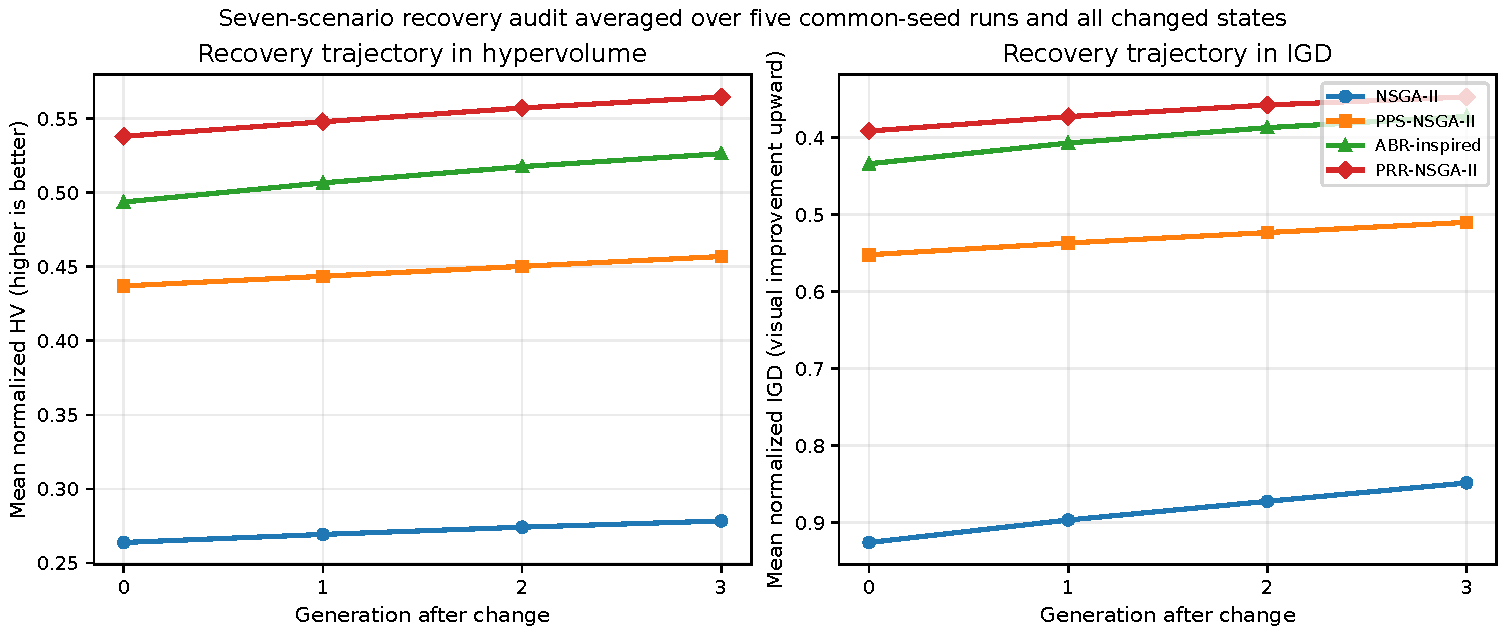
\includegraphics[width=\linewidth]{recovery_curves_HV_IGD.pdf}
\caption{Change-response recovery curves for the seven-scenario manuscript-facing recovery audit. Generation~0 is the population immediately after the response step; generations~1--3 are the subsequent evolutionary generations. The HV panel shows mean normalized hypervolume. The IGD panel shows scenario-normalized IGD (lower raw values are better), with the axis inverted so that upward movement indicates better recovery. Averages are computed over five common-seed runs and all changed states in the audit protocol.}
\label{fig:recovery-curves}
\end{figure}

The recovery diagnostic supports the bounded claim. NSGA-II has no response gain and recovers slowly. PPS-NSGA-II gains immediately from direct prediction, but its three-generation gain is lower than ABR and PRR. Under the reproduced five-run diagnostic, PRR-NSGA-II gives the largest immediate response gain, the largest three-generation recovery gain, the steepest recovery slope, and the shortest mean time-to-threshold among the four inspected methods. The new generation-wise curves make the same pattern visually explicit. This directly supports the rapid-recovery interpretation: PRR is not the strongest overall adaptive controller in the full main experiment, but it provides a conservative response that recovers quickly in the tested stress/application diagnostic while retaining selection-filtered admission.


\subsection{Source-admission diagnostics}
The central mechanism of PRR is not the size of the proposal blocks, but the source composition that survives current-state environmental selection. Therefore, Table~\ref{tab:source-acceptance-type} and Figure~\ref{fig:source-acceptance-type} move the source-diagnostic evidence from the supplementary material into the main results. The table reports the accepted population share of elite, memory, prediction, and diversity candidates after filtering. These shares are outcomes of selection, not preallocated quotas. For example, prediction candidates account for only $19.9\%$ of the accepted redeployed population in high-severity cases, but rise to $38.6\%$ in high-frequency cases. Conversely, elite candidates remain dominant overall but are reduced in the high-frequency subset. This pattern supports the intended interpretation: PRR does not force a fixed number of predicted, memory, or elite candidates into the next population; it exposes all sources to the same current-state admission test and lets the accepted composition vary with the dynamic regime.

\begin{table}[htbp]
\centering
\caption{Accepted PRR candidate-source composition after current-state environmental selection. Values are mean shares of the redeployed population, in percent, aggregated over PRR response events. The proposal pool is larger than the population, so these are observed admission outcomes rather than fixed quotas.}
\label{tab:source-acceptance-type}
\scriptsize
\setlength{\tabcolsep}{4pt}
\renewcommand{\arraystretch}{1.12}
\begin{tabular}{lrrrrrr}
\toprule
Scenario type & Scen. & Events & Elite & Memory & Prediction & Diversity \\
 & & & \multicolumn{4}{c}{Accepted population share (\%)} \\
\midrule
Regular & 11 & 6270 & 55.6 & 18.6 & 24.8 & 1.0 \\
High-frequency & 3 & 1710 & 46.0 & 14.9 & 38.6 & 0.5 \\
High-severity & 3 & 1710 & 58.9 & 21.0 & 19.9 & 0.3 \\
Low-frequency & 1 & 570 & 51.8 & 16.9 & 31.1 & 0.2 \\
Application-inspired & 2 & 1140 & 55.3 & 17.5 & 26.9 & 0.3 \\
\midrule
\textbf{All scenarios} & 20 & 11400 & 54.4 & 18.2 & 26.7 & 0.7 \\
\bottomrule
\end{tabular}
\end{table}

\begin{figure}[htbp]
\centering
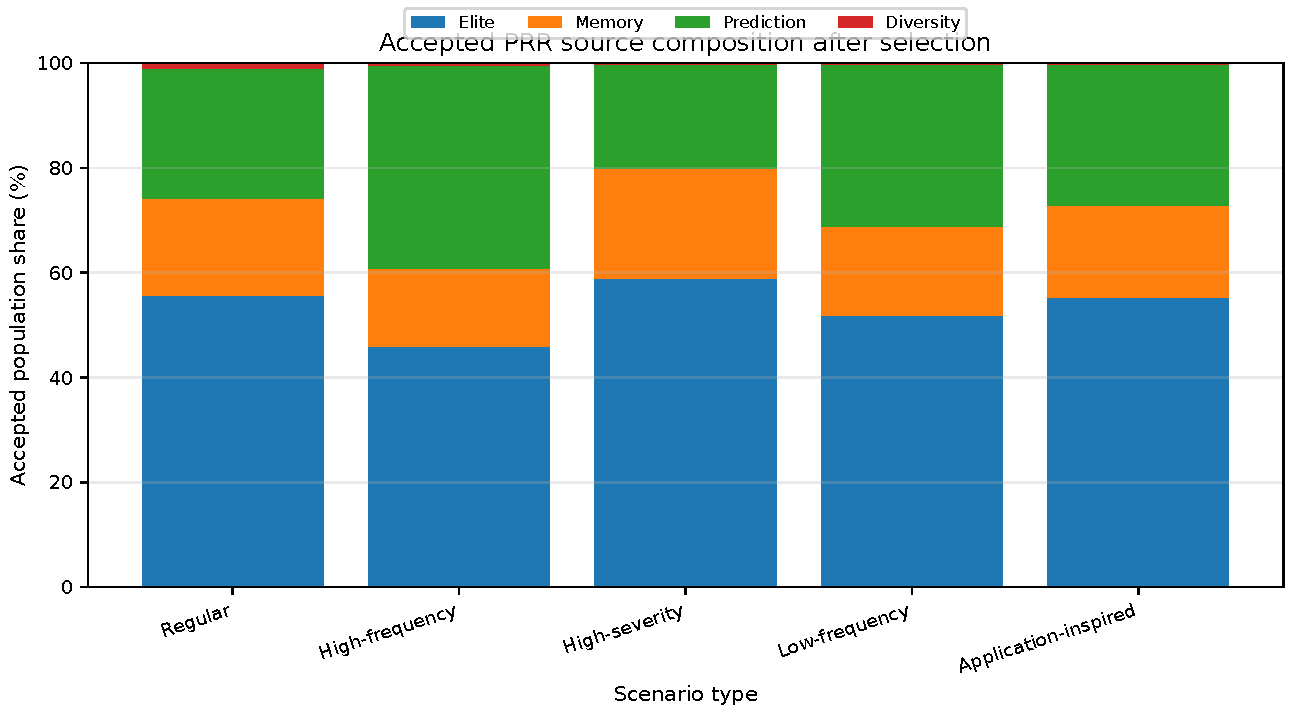
\includegraphics[width=0.92\linewidth]{source_acceptance_by_type.pdf}
\caption{Accepted PRR candidate-source composition by scenario type. Each stacked bar sums to the accepted redeployed population after current-state environmental selection. The variation across scenario types shows that PRR's fixed proposal blocks do not translate into fixed admission shares.}
\label{fig:source-acceptance-type}
\end{figure}

\subsection{Ablation and component-risk analysis}
Table \ref{tab:ablation} and Figure \ref{fig:ablation-hv} report the component-removal and direct-insertion ablations across all 20 scenarios and 30 runs under the same three-generation-per-state rapid-response budget used in the main protocol. To avoid treating the complete PRR configuration as a separate ablation setting, the PRR-complete row is now taken from the same raw runs as the main PRR-NSGA-II row and renamed only for the ablation table. A consistency audit in the supplementary results verifies zero numerical difference between main PRR-NSGA-II and PRR-complete for all five metrics. Therefore, the ablation baseline is exactly the main method rather than a different seed stream or generation budget.

The ablation should not be interpreted as evidence that the full fixed-quota PRR configuration is uniformly best. It shows a more nuanced component-risk behavior. Removing prediction causes the clearest collapse, decreasing normalized HV from $0.512$ to $0.378$ and increasing IGD from $0.244$ to $0.486$; thus, temporal movement estimation is the dominant recovery source in this rapid-response setting. By contrast, the no-memory, no-diversity, and no-elite variants can improve aggregate HV or IGD under this benchmark mix. This result identifies the main operational risk of the proposed design: when environments do not recur strongly, when archived regions become stale, or when diversity pressure is already supplied by mutation and environmental change, fixed memory, elite, or diversity proposal shares can become non-optimal. Memory assistance should therefore be read as an available candidate source in the redeployment pool, not as an unconditional guarantee that forcing more memory-derived proposals improves every scenario.

The direct-insertion variant is retained as a stress test rather than as a proof that filtering wins on every aggregate mean. Under the matched three-generation protocol, direct insertion is close to PRR-complete and slightly better on the aggregate HV and IGD means ($0.519$ versus $0.512$ HV and $0.233$ versus $0.244$ IGD). This boundary condition is important: if prediction is accurate enough, reserved insertion can be competitive. The value of PRR's admission filter is instead its safety interpretation. Predicted candidates are not guaranteed protected slots; they must survive current-state selection against elite, memory/transfer, and diversity candidates. The controlled prediction-noise stress test below therefore remains the more direct verification of the intended contamination-control mechanism.

The revised supplementary package includes complete machine-readable ablation outputs for all 20 benchmark scenarios: raw run metrics, per-scenario means and standard deviations, average ranks, win/tie/loss counts against PRR-complete, the scenario-metric winner for each ablation variant, protocol metadata, and a main-PRR versus PRR-complete consistency audit. This makes the ablation a diagnostic component-risk analysis rather than a selective demonstration that every added component always helps.

\begin{figure}[htbp]
\centering
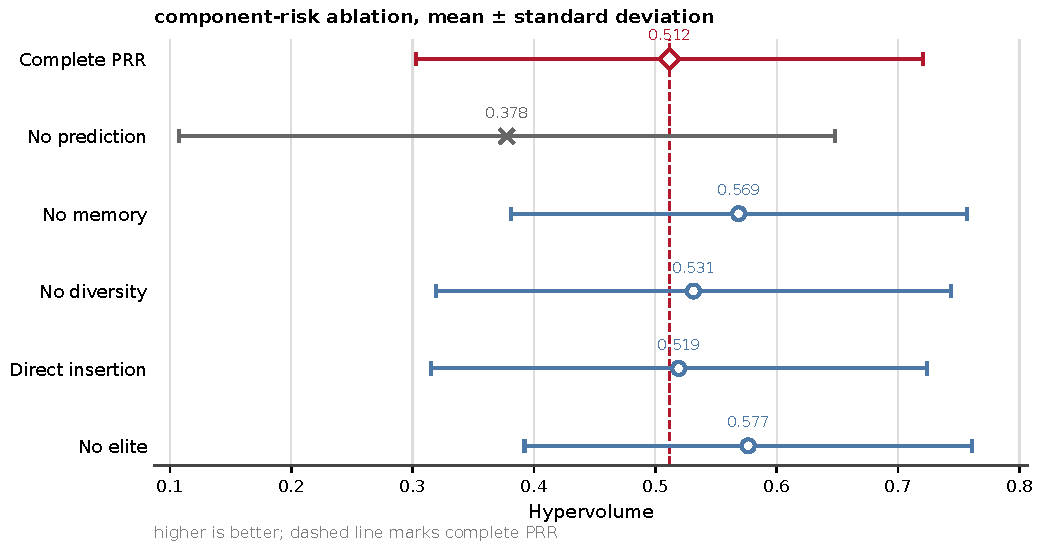
\includegraphics[width=0.95\linewidth]{ablation_hv.pdf}
\caption{All-scenario ablation results for hypervolume with mean $\pm$ standard-deviation intervals; the dashed reference marks the complete PRR configuration.}
\label{fig:ablation-hv}
\end{figure}

\subsection{Sensitivity and stress analysis}
Sensitivity analysis was conducted for generations per state, population size, decision dimensionality, prediction history length (recent centroids), prediction scale, PRR source shares, and the recent/transfer memory split. Table \ref{tab:sens-generations} shows that increasing the number of generations per state improves HV, IGD, stability, and QDR. Thus, the main setting should be interpreted as a deliberately difficult rapid-recovery profile rather than the only valid operating regime.

\begin{table}[htbp]
\centering
\caption{Sensitivity of PRR-NSGA-II to the number of generations per environmental state.}
\label{tab:sens-generations}
\begin{tabular}{lrrrr}
\toprule
Generations & HV & IGD & Stability & QDR \\
\midrule
3 & 0.404 & 0.235 & 0.956 & 0.328 \\
5 & 0.438 & 0.202 & 0.958 & 0.364 \\
10 & 0.507 & 0.124 & 0.965 & 0.429 \\
20 & 0.567 & 0.062 & 0.974 & 0.484 \\
\bottomrule
\end{tabular}
\end{table}

To avoid leaving the method only at $D=10$, Table~\ref{tab:scalability-diagnostic} adds a compact dimensional scalability diagnostic. The diagnostic repeats the same rapid-response setting at $D=10$ and $D=30$ on six representative scenarios: FDA1, dMOP2, DF1-HF, FDA1-HS, dMOP2-HS, and APP-RESOURCE. It uses four representative methods and five common-seed runs rather than the full 20-scenario, 10-algorithm, 30-run suite; it should therefore be read as a scalability check, not as a complete high-dimensional benchmark. The population size is kept fixed at $N=100$ to isolate the effect of increasing the decision dimension. Absolute approximation quality degrades at $D=30$, as expected under the same short three-generation response budget, but PRR-NSGA-II retains the best average HV, IGD, QDR, and scenario-level HV/IGD ranks among the four inspected methods. This supports the claim that the selection-filtered redeployment mechanism is not merely a $D=10$ artifact, while a broader large-scale study remains necessary.

\begin{table}[htbp]
\centering
\caption{Compact dimensional scalability diagnostic on six representative scenarios. The diagnostic is not a full high-dimensional rerun; it repeats the rapid-response protocol for five common-seed runs at $D=10$ and $D=30$ using four representative methods. HV and QDR are maximized, IGD is minimized, and ranks are scenario-level averages over the six diagnostic scenarios.}
\label{tab:scalability-diagnostic}
\scriptsize
\setlength{\tabcolsep}{3pt}
\begin{tabular}{llrrrrr}
\toprule
$D$ & Method & HV & IGD & QDR & HV rank & IGD rank \\
\midrule
10 & NSGA-II & 0.218 & 1.116 & 0.181 & 4.00 & 4.00 \\
10 & PPS-NSGA-II & 0.446 & 0.307 & 0.379 & 2.17 & 2.33 \\
10 & ABR-inspired & 0.495 & 0.189 & 0.410 & 2.50 & 2.33 \\
10 & PRR-NSGA-II & \textbf{0.526} & \textbf{0.157} & \textbf{0.443} & \textbf{1.33} & \textbf{1.33} \\
\midrule
30 & NSGA-II & 0.147 & 5.011 & 0.117 & 4.00 & 4.00 \\
30 & PPS-NSGA-II & 0.184 & 1.609 & 0.132 & 2.17 & 2.33 \\
30 & ABR-inspired & 0.159 & 1.660 & 0.117 & 2.83 & 2.67 \\
30 & PRR-NSGA-II & \textbf{0.220} & \textbf{1.060} & \textbf{0.158} & \textbf{1.00} & \textbf{1.00} \\
\bottomrule
\end{tabular}
\end{table}

Table \ref{tab:quota-sensitivity} reports a targeted 8-scenario, 12-run source-quota audit on representative smooth, high-frequency, high-severity, adapted DF-style, and application-inspired cases. This diagnostic audit is deliberately smaller than the main 20-scenario, 30-run comparison and is used only to test whether the default shares are harmless constants. They are not. Lower elite or higher prediction shares improve HV on this subset, whereas overly low prediction, overly high memory, or high elite preservation reduce approximation quality. This supports the revised interpretation of PRR: the admission filter is the methodological contribution, while the fixed source shares are tunable design parameters and should eventually be made adaptive.

Table \ref{tab:prediction-noise-stress} gives a synthetic stress test for the selection-filtered admission rule. When prediction noise increases, PRR sharply reduces the number of accepted predicted candidates, while direct insertion continues to force 25 predicted candidates. The direct-insertion contamination count rises with prediction error, whereas the filtered rule admits no harmful predicted candidates under this diagnostic definition. This experiment does not prove superiority on every benchmark; it verifies the intended safety mechanism under controlled prediction error and motivates the Discussion interpretation that PRR is most useful when prediction reliability varies rather than when prediction is uniformly accurate.

\begin{table}[htbp]
\centering
\caption{Targeted 8-scenario, 12-run PRR source-quota sensitivity audit. The table reports mean HV, IGD, and QDR over 12 independent runs per representative scenario while varying the elite, memory, prediction, diversity, and recent-memory split parameters under the same selection-filtered admission rule. Lower IGD is better; higher HV and QDR are better.}
\label{tab:quota-sensitivity}
\scriptsize
\resizebox{\textwidth}{!}{%
\begin{tabular}{lrrrrrrrr}
\toprule
Variant & $q_e$ & $q_m$ & $q_p$ & $q_d$ & $r_m$ & HV & IGD & QDR \\
\midrule
Default & 0.35 & 0.30 & 0.25 & 0.10 & 0.55 & 0.561 & 0.239 & 0.472 \\
Low elite & 0.20 & 0.30 & 0.35 & 0.15 & 0.55 & 0.587 & 0.206 & 0.494 \\
High elite & 0.50 & 0.22 & 0.20 & 0.08 & 0.55 & 0.547 & 0.265 & 0.460 \\
Low memory & 0.40 & 0.15 & 0.35 & 0.10 & 0.55 & 0.574 & 0.224 & 0.484 \\
High memory & 0.25 & 0.45 & 0.20 & 0.10 & 0.55 & 0.553 & 0.252 & 0.465 \\
Low prediction & 0.45 & 0.35 & 0.10 & 0.10 & 0.55 & 0.513 & 0.317 & 0.434 \\
High prediction & 0.25 & 0.25 & 0.40 & 0.10 & 0.55 & 0.579 & 0.217 & 0.489 \\
Low diversity & 0.38 & 0.32 & 0.28 & 0.02 & 0.55 & 0.545 & 0.279 & 0.461 \\
High diversity & 0.25 & 0.25 & 0.25 & 0.25 & 0.55 & 0.578 & 0.216 & 0.485 \\
Recent-heavy memory & 0.35 & 0.30 & 0.25 & 0.10 & 0.80 & 0.556 & 0.249 & 0.468 \\
Transfer-heavy memory & 0.35 & 0.30 & 0.25 & 0.10 & 0.25 & 0.564 & 0.241 & 0.475 \\
\bottomrule
\end{tabular}%
}
\vspace{0.5ex}
\footnotesize{Targeted diagnostic audit: 8 representative scenarios $\times$ 12 independent runs per scenario/variant. $r_m$ is the recent-memory share inside the memory/transfer component; $1-r_m$ is the historical-transfer share.}
\end{table}
\begin{table}[htbp]
\centering
\caption{Synthetic prediction-noise stress test. PRR admits predicted candidates only if they survive current-state selection, whereas direct insertion reserves 25 predicted slots. Contaminated predictions are retained predicted candidates worse than the $N$th non-predicted alternative in the same pool.}
\label{tab:prediction-noise-stress}
\scriptsize
\setlength{\tabcolsep}{4pt}
\resizebox{\textwidth}{!}{%
\begin{tabular}{rrrrrr}
\toprule
Noise & PRR accepted pred. & Direct forced pred. & PRR contaminated & Direct contaminated & Direct priority loss \\
\midrule
0.00 & 25.16 & 25.00 & 0.00 & 0.81 & 0.278 \\
0.03 & 8.81 & 25.00 & 0.00 & 10.96 & 0.298 \\
0.06 & 2.46 & 25.00 & 0.00 & 21.80 & 0.323 \\
0.10 & 0.52 & 25.00 & 0.00 & 24.43 & 0.335 \\
0.15 & 0.14 & 25.00 & 0.00 & 24.84 & 0.339 \\
0.20 & 0.06 & 25.00 & 0.00 & 24.93 & 0.341 \\
0.30 & 0.02 & 25.00 & 0.00 & 24.98 & 0.341 \\
\bottomrule
\end{tabular}%
}
\end{table}


\section{Discussion}
The experiments support six observations. First, PRR-NSGA-II remains competitive on the expanded dynamic benchmark set, but the ABR-inspired implementation is the strongest overall adaptive competitor and should be treated as the current reference point for this controlled implementation. Second, the evaluation-count audit shows that equal generations per state do not imply equal objective-vector evaluations; therefore, the claims are framed around equal-generation rapid response, scenario-level ranks, and diagnostic recovery behavior rather than strict equal-function-evaluation superiority. Third, the baseline comparison is now transparent: every compared method has a stated response family, quota policy, archive rule, and pseudocode in the supplementary material, while the manuscript explicitly avoids claiming bitwise reproduction of all original author code. Fourth, PRR-NSGA-II consistently outperforms static, immigrant, memory-only, decomposition, transfer, and robust-response baselines on most approximation-quality comparisons. Fifth, PPS-NSGA-II and the ABR-inspired implementation show that direct prediction insertion and adaptive response allocation can be highly effective on regular FDA, dMOP, and adapted DF-style dynamics. Sixth, the subgroup, family, and ablation analyses clarify why the method is still publishable despite not being the overall mean winner: PRR is first on the high-frequency subset and on the application-inspired subset for the main quality indicators, remains close to the ABR-inspired variant on scenario-normalized HV/IGD/QDR scores, and is weaker on high-severity and prediction-hostile/adaptive-favored settings where response allocation or direct prediction is more effective. The ablation study identifies prediction as the most influential PRR component for approximation recovery, but it also exposes a component-risk trade-off: memory and elite preservation can be neutral or harmful when old environments do not recur or when previous elites become stale after abrupt movement. This weakens any unconditional claim that the full configuration must dominate all simplified variants, but it strengthens the methodological interpretation of PRR as a transparent redeployment framework whose candidate sources can be inspected, removed, or adaptively weighted.

The ABR-inspired implementation deserves separate interpretation because it is not merely another baseline in the table; it explains the main limitation of PRR. In this implementation, the ABR-inspired variant keeps an elite block but generates full memory, prediction, and diversity candidate pools, evaluates them in the current environment, scores the pools, and adaptively allocates the remaining response budget. This online allocation can outperform PRR's fixed nominal $0.35/0.30/0.25/0.10$ generation-share vector, which is realized as an over-generated $2N$ pool before selection, when the usefulness of memory, prediction, and diversity changes from one state to the next. In high-severity or prediction-hostile cases, the ABR-inspired variant can shift budget away from misleading prediction or stale memory and toward the source with better current-state scores. PRR instead uses a conservative admission filter but fixed candidate-generation shares; if too much of the over-generated candidate pool is assigned to a temporarily weak source, environmental selection can reject poor candidates, but it cannot recover the opportunity cost of not generating more candidates from a better source. This is the most plausible reason the ABR-inspired variant leads the overall means and ranks first on IGD and QDR.

The same comparison also identifies a concrete next step rather than only a weakness. PRR and ABR-style allocation are complementary: adaptive boosting changes the amount of each response source, whereas PRR controls whether generated candidates receive reserved admission. A natural extension is therefore adaptive PRR, in which prediction, memory, transfer, elite, and diversity quotas are chosen by confidence scores, recent accepted-candidate rates, or candidate-pool quality before the final selection-filtered admission step. Such a design would preserve PRR's safeguard against forced prediction insertion while reducing the fixed-quota penalty observed in high-severity and prediction-hostile subsets. The new quota-sensitivity audit supports this direction: prediction-heavy and lower-elite configurations can improve approximation quality on representative rapid-change cases, while memory-heavy and prediction-low settings can amplify negative transfer. Therefore, the fixed $0.35/0.30/0.25/0.10$ share vector should be read as a transparent default for generating the $2N$ proposal pool, not as an optimized universal setting or as final admission quotas.

The methodological contribution should therefore be interpreted as an admission-control design, not as a claim that filtering always maximizes HV in every smooth scenario. PRR-NSGA-II does not replace NSGA-II environmental selection; it deliberately prevents prediction from bypassing that selection. Prediction, diversity, elite preservation, and the internally split memory block are all treated as competing candidate sources for the new environment. This framing is important because many prediction-based DMOEAs differ primarily in how they generate candidate movement, whereas PRR focuses on how predicted candidates are admitted after re-evaluation. The conservative admission property in Section 4 makes this distinction explicit: a low-priority predicted candidate cannot be forced into $P^{PRR}_t$ if the evaluated union contains $N$ better alternatives. The property is simple by construction, but this simplicity is the intended safeguard. It prevents the method from over-committing to a wrong movement estimate while keeping the prediction operator available when movement estimation is helpful. The prediction-noise stress test should be read in exactly this way. PRR's advantage is not expected when prediction accuracy is uniformly high; in that case, reserved insertion can be equally good or better. Its advantage emerges when prediction reliability is variable across states or scenario families, because the filter can admit accurate predicted candidates in informative states while rejecting contaminated predicted candidates when the movement estimate becomes unreliable. Thus the stress test is not an auxiliary experiment detached from the main claim; it is the most direct diagnostic of the paper's central mechanism, namely selection-filtered admission under uncertain prediction quality.

The results also delimit the scope of the claim. Direct insertion is not inherently inferior; when the environment is smooth and prediction is accurate, reserved predicted candidates can accelerate convergence and sometimes achieve slightly higher HV. Memory assistance is also not inherently beneficial; when the dynamic process does not revisit similar Pareto-set regions, archived candidates can act as negative transfer unless their admission is filtered or their quota is adapted. Elite preservation has the same limitation because previous elites may be high-quality historical points rather than useful current-state seeds. The ABR-inspired implementation further shows that adaptive response allocation is a very strong overall baseline. PRR-NSGA-II is therefore best described as a conservative, interpretable, and modular soft-computing redeployment alternative rather than as an overall SOTA replacement for adaptive boosting. Its strongest empirical justification comes from high-frequency and application-inspired settings, where current-state filtering keeps useful predicted movement while preventing prediction from receiving guaranteed admission. Its weaker cases are equally informative: high-severity changes and prediction-hostile/adaptive-favored profiles indicate that the fixed PRR source ratios should be replaced in future work by adaptive quota control and prediction-confidence estimation.

\section{Threats to Validity}
The benchmark suite now includes FDA, dMOP, and adapted DF-style cases, but the study is still limited to two-objective continuous problems. The two application-inspired APP cases are synthetic diagnostics, not real-world validated datasets; they improve practical relevance by adding stylized resource-allocation and scheduling dynamics, but they do not replace validation on real operational data. Real-world dynamic decision problems may include constraints, noise, discontinuous changes, many objectives, mixed variables, expensive evaluations, or human preferences. The compared adaptive, transfer, decomposition, and robust-response baselines are implemented in one reproducible code base and are documented with method-level pseudocode and parameter tables, but they are still not exact source-code reproductions of every original method. This limitation is important for ABR, ARVLP, KTR, and related recent methods whose original implementations may include additional engineering choices, tuning, or benchmark-specific details. The results should therefore be read as controlled response-family evidence under a common implementation, not as a final ranking of every original algorithm package. The main-text FE-accounting table and supplementary evaluation audit show that the main experiment is an equal-generation protocol rather than a strict equal-function-evaluation protocol; a full FE-capped rerun should be added in future work if strict FE parity is required by the target venue. The added $D=30$ diagnostic reduces the risk that the evidence is purely $D=10$-specific, but it remains a compact six-scenario, four-method check rather than a full large-scale study. The main experiment emphasizes rapid recovery under a small generation budget; the sensitivity, quota, stress, scalability, and recovery diagnostics show that performance improves as the budget increases, that source shares affect performance, that dimensionality increases difficulty, and that response operators differ in immediate post-change recovery. Future work should include JY-style, constrained, many-objective, large-scale, real-data dynamic benchmarks, and direct comparisons against any publicly available original author implementations.

\section{Conclusion}
This paper presented PRR-NSGA-II, a selection-filtered predictive redeployment strategy with bounded memory support for dynamic multi-objective evolutionary optimization within an evolutionary soft-computing framework. The main methodological contribution is selection-filtered candidate admission: temporal prediction generates candidates, but current-state environmental selection decides how many predicted candidates, if any, enter the redeployed population. The method uses four candidate-generation blocks--elite, memory, prediction, and diversity--with recent-memory and historical-transfer sampling represented as internal sub-blocks of memory, and it applies selection-filtered redeployment without giving any response source reserved admission to the next population. Experiments on 20 FDA, dMOP, adapted DF-style, stress-variant, and application-inspired synthetic diagnostic scenarios show that PRR-NSGA-II is a strong but not dominant competitor among 10 algorithms in the tested equal-generation rapid-recovery setting. The ABR-inspired implementation remains the strongest overall adaptive reference point on most mean indicators, whereas PRR-NSGA-II provides a conservative and interpretable alternative that is especially competitive in high-frequency and application-inspired subsets, ranks first on scenario-level HV and stability, and remains close to the ABR-inspired variant on scenario-normalized approximation-quality scores. High-severity and prediction-hostile/adaptive-favored results identify the main limitation: fixed conservative admission should be complemented by adaptive quota control when the usefulness of prediction changes sharply across environments. Ablation results confirm that prediction is the dominant contributor to approximation recovery, but they also show that memory and elite preservation require careful quota control because they can become negative-transfer sources when the environment does not revisit earlier regions. The direct-insertion test and QDR expose the trade-off between active recovery, conservative admission, and compromise consistency. Future work will extend the framework to constrained and many-objective optimization, preference-aware decision support, adaptive prediction-confidence control, and real-world dynamic scheduling or resource-allocation data.


\section*{CRediT authorship contribution statement}
Ercan Erkalkan: Conceptualization, Methodology, Software, Validation, Formal analysis, Investigation, Data curation, Writing--original draft, Writing--review and editing, Visualization.

\section*{Data availability}
The supplementary reproducibility archive accompanying this manuscript contains the Python implementation, raw results, summary tables, statistical-test outputs, figures, run scripts, benchmark-definition supplement, baseline-implementation supplement, objective-evaluation audit, and PRR accepted-source diagnostic files. The LaTeX source, BibTeX database, input tables, and manuscript figures required to rebuild the submitted PDF are provided separately in the submission source package. The public experiment-code release is archived on Zenodo at \url{https://doi.org/10.5281/zenodo.20327988}. The corresponding GitHub repository is available at \url{https://github.com/ErcanErkalkan/Memory-Assisted-Predictive-Redeployment}.

\section*{Funding}
This research received no external funding.

\section*{Ethics statement}
Not applicable. This study uses benchmark functions and does not involve human participants, animals, or personally identifiable data.

\section*{Declaration of competing interest}
The author declares that there are no known competing financial interests or personal relationships that could have appeared to influence the work reported in this paper.

\section*{Declaration of generative AI and AI-assisted technologies in the writing process}
During the preparation of this work, the author used generative AI assistance for language editing, LaTeX drafting support, and formatting support. The author reviewed and edited the content as needed and takes full responsibility for the content of the published article.

{\small
\bibliographystyle{elsarticle-num}
\bibliography{ASC_PRR_NSGAII_references}
}
\end{document}
